% Suggested time: 2-3 minutes
\section{Graph Model and Data}

\begin{frame}{Vertices: \NumVertices{} Locations in Cagayan de Oro}
  \centering
  \scriptsize
  \renewcommand{\arraystretch}{0.92}
  % AUTO-GENERATED by code/main.py --export-latex. Do not edit; re-run the export instead.
\begin{tabular}{l l l r r}
\toprule
\textbf{Vertex} & \textbf{Location} & \textbf{Area} & \textbf{Latitude} & \textbf{Longitude} \\
\midrule
V0 & USTP Cagayan de Oro Campus (start) & C. M. Recto Ave, Lapasan & 8.48607 & 124.65681 \\
V1 & Limketkai Center & Lapasan & 8.48139 & 124.65637 \\
V2 & Centrio Mall & C. M. Recto Ave, Licoan & 8.48483 & 124.65062 \\
V3 & Pelaez Sports Center & Don Apolinar Velez St, Burgos & 8.48180 & 124.64702 \\
V4 & Museo de Oro (Xavier University) & Corrales Ave, Nazareth & 8.47587 & 124.64598 \\
V5 & Divisoria Plaza & Barangay 5, Carmen & 8.47750 & 124.64465 \\
V6 & St. Augustine Metropolitan Cathedral & Gaston Circle, Carmen & 8.47497 & 124.64147 \\
V7 & Port of Cagayan de Oro & Macabalan & 8.49453 & 124.66219 \\
V8 & Liceo de Cagayan University & R. N. Pelaez Blvd, Carmen & 8.48566 & 124.63927 \\
V9 & Capitol University & Corrales Ext, Barangay 25 & 8.48818 & 124.65257 \\
\bottomrule
\end{tabular}

  \medskip
  \raggedright\footnotesize
  Coordinates: OpenStreetMap / Nominatim~\cite{osm}, located on Google Maps~\cite{googlemaps}.
\end{frame}

\begin{frame}{The Weighted Graph $G = K_{\NumVertices}$}
  \centering
  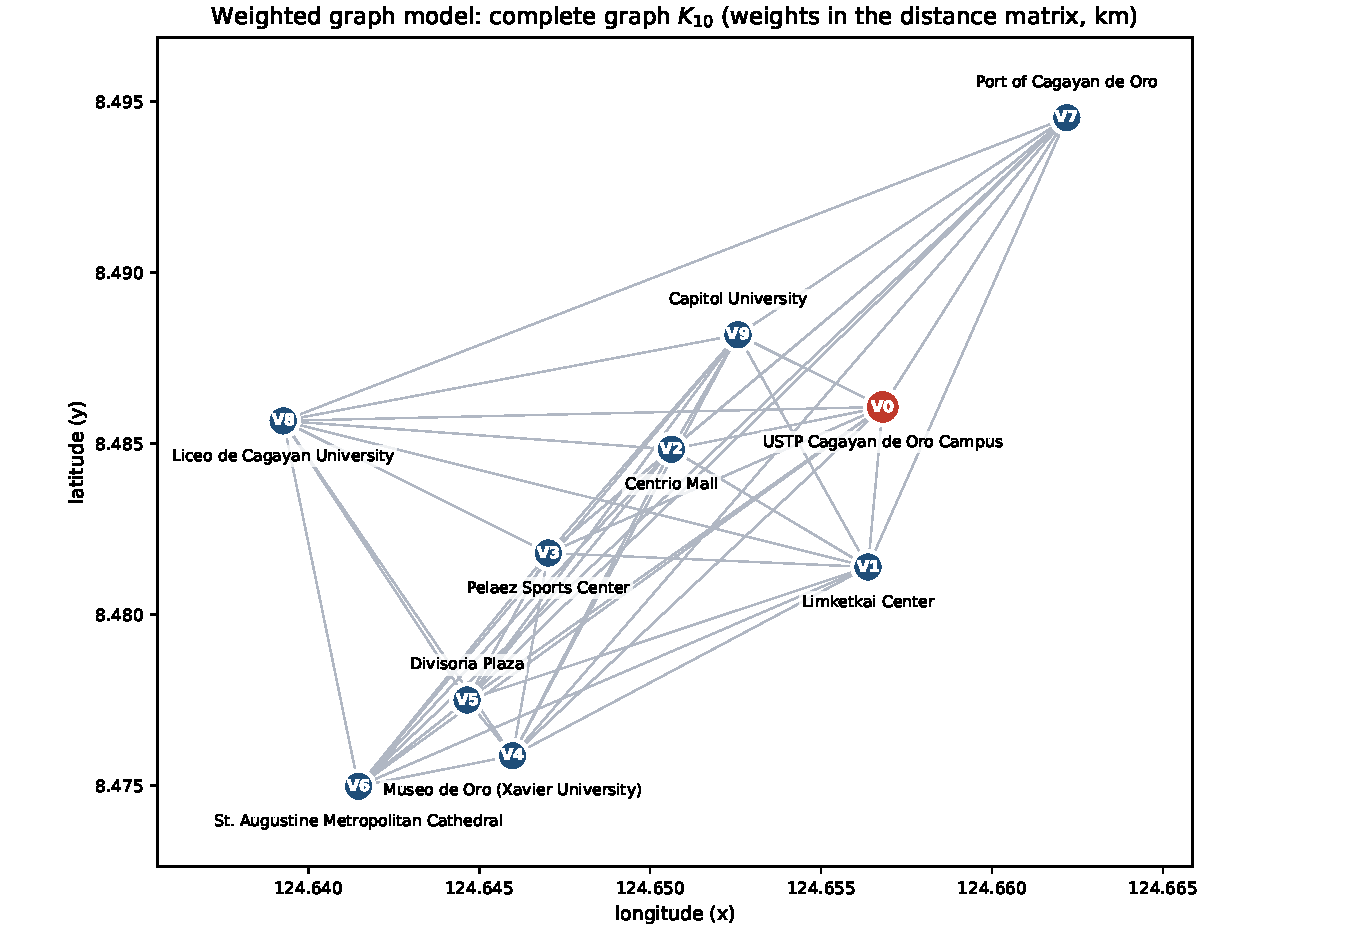
\includegraphics[height=0.78\textheight]{graph.pdf}

  \footnotesize Complete graph: \NumEdges{} edges, one for each pair of locations; each edge is the
  driving route OSRM returns between them (it may pass other stops without visiting them).
\end{frame}

\begin{frame}{Edges, Direction and Weights}
  \begin{columns}[T]
    \begin{column}{0.62\textwidth}
      \centering
      \resizebox{\linewidth}{!}{% AUTO-GENERATED by code/main.py --export-latex. Do not edit; re-run the export instead.
\begin{tabular}{l rrrrrrrrrr}
\toprule
 & \textbf{V0} & \textbf{V1} & \textbf{V2} & \textbf{V3} & \textbf{V4} & \textbf{V5} & \textbf{V6} & \textbf{V7} & \textbf{V8} & \textbf{V9} \\
\midrule
\textbf{V0} & -- & 1.09 & 1.26 & 1.94 & 2.48 & 2.37 & 2.83 & 2.07 & 2.62 & 1.34 \\
\textbf{V1} & 1.09 & -- & 1.55 & 2.24 & 2.10 & 2.21 & 2.50 & 2.32 & 2.96 & 1.68 \\
\textbf{V2} & 1.26 & 1.55 & -- & 1.18 & 1.55 & 1.61 & 1.85 & 2.17 & 1.86 & 0.58 \\
\textbf{V3} & 1.94 & 2.24 & 1.18 & -- & 1.31 & 0.97 & 1.43 & 2.98 & 2.15 & 1.38 \\
\textbf{V4} & 2.48 & 2.10 & 1.55 & 1.31 & -- & 0.54 & 0.87 & 3.52 & 1.92 & 1.93 \\
\textbf{V5} & 2.37 & 2.21 & 1.61 & 0.97 & 0.54 & -- & 0.74 & 3.29 & 1.58 & 1.70 \\
\textbf{V6} & 2.83 & 2.50 & 1.85 & 1.43 & 0.87 & 0.74 & -- & 3.87 & 1.65 & 2.28 \\
\textbf{V7} & 2.07 & 2.32 & 2.17 & 2.98 & 3.52 & 3.29 & 3.87 & -- & 3.66 & 1.79 \\
\textbf{V8} & 2.62 & 2.96 & 1.86 & 2.15 & 1.92 & 1.58 & 1.65 & 3.66 & -- & 2.06 \\
\textbf{V9} & 1.34 & 1.68 & 0.58 & 1.38 & 1.93 & 1.70 & 2.28 & 1.79 & 2.06 & -- \\
\bottomrule
\end{tabular}
}

      \scriptsize $w(i,j)$ = road distance in \textbf{km}
    \end{column}
    \begin{column}{0.36\textwidth}
      \footnotesize
      \textbf{Undirected:} one-way streets make raw distances differ slightly, so
      \[ w(u,v) = \tfrac12\bigl(d(u{\to}v) + d(v{\to}u)\bigr) \]
      \textbf{Actual data:} locations; road distances from the OSRM Table service~\cite{osrmapi}
      on the OpenStreetMap road network~\cite{luxen2011osrm}.

      \textbf{Assumed:} symmetric averaging; no traffic or time windows; choice of stops.
    \end{column}
  \end{columns}
\end{frame}

\begin{frame}{Cross-Check with Google Maps}
  \begin{columns}[T]
    \begin{column}{0.55\textwidth}
      \centering
      \scriptsize
      \setlength{\tabcolsep}{4pt}
      \begin{tabular}{c l r r r}
        \toprule
        \textbf{Leg} & \textbf{From $\to$ To} & \textbf{Matrix} & \textbf{Google} & \textbf{\%} \\
        \midrule
        1 & V0 $\to$ V1 & 1.09 & 0.70 & $-36$ \\
        2 & V1 $\to$ V7 & 2.32 & 3.10 & $+34$ \\
        3 & V7 $\to$ V9 & 1.79 & 2.00 & $+12$ \\
        4 & V9 $\to$ V2 & 0.58 & 0.65 & $+12$ \\
        5 & V2 $\to$ V3 & 1.18 & 1.10 & $-7$ \\
        6 & V3 $\to$ V4 & 1.31 & 1.70 & $+30$ \\
        7 & V4 $\to$ V5 & 0.54 & 0.70 & $+30$ \\
        8 & V5 $\to$ V6 & 0.74 & 0.45 & $-39$ \\
        9 & V6 $\to$ V8 & 1.65 & 1.60 & $-3$ \\
        10 & V8 $\to$ V0 & 2.62 & 2.40 & $-8$ \\
        \midrule
        & \textbf{Total} & \textbf{13.82} & \textbf{14.40} & $+4.2$ \\
        \bottomrule
      \end{tabular}
    \end{column}
    \begin{column}{0.42\textwidth}
      \footnotesize
      Each leg of our route searched separately on Google Maps~\cite{googlemaps} in driving mode.
      \medskip

      \textbf{Whole tour:} within \textbf{4.2\%}.

      \textbf{Single legs:} differ by up to 39\% (pin positions, one-way streets, different road
      choices and turn restrictions).
      \medskip

      We keep the OSRM matrix: it is reproducible and read directly by the program.
    \end{column}
  \end{columns}
\end{frame}

\begin{frame}{Applying the Algorithm: Divide (seed \DCSeed{})}
  \centering
  \resizebox{0.95\textwidth}{!}{% AUTO-GENERATED by code/main.py --export-latex. Do not edit; re-run the export instead.
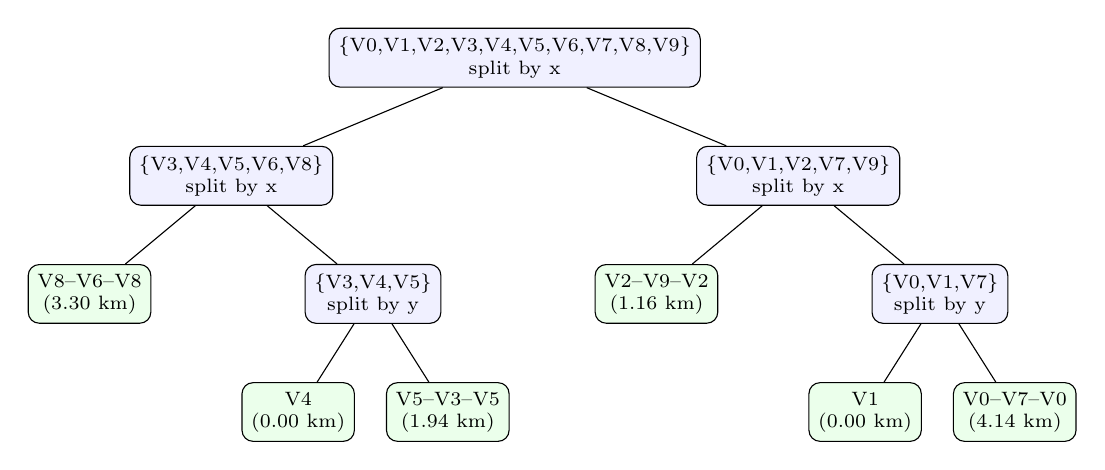
\begin{tikzpicture}[
  split/.style={draw, rounded corners, fill=blue!6, align=center, font=\scriptsize},
  leaf/.style={draw, rounded corners, fill=green!8, align=center, font=\scriptsize},
  level 1/.style={sibling distance=7.2cm, level distance=1.5cm},
  level 2/.style={sibling distance=3.6cm, level distance=1.5cm},
  level 3/.style={sibling distance=1.9cm, level distance=1.5cm}]
\node[split] {\{V0,V1,V2,V3,V4,V5,V6,V7,V8,V9\}\\split by x}
  child {
    node[split] {\{V3,V4,V5,V6,V8\}\\split by x}
    child {
      node[leaf] {V8--\allowbreak V6--\allowbreak V8\\(3.30 km)}
    }
    child {
      node[split] {\{V3,V4,V5\}\\split by y}
      child {
        node[leaf] {V4\\(0.00 km)}
      }
      child {
        node[leaf] {V5--\allowbreak V3--\allowbreak V5\\(1.94 km)}
      }
    }
  }
  child {
    node[split] {\{V0,V1,V2,V7,V9\}\\split by x}
    child {
      node[leaf] {V2--\allowbreak V9--\allowbreak V2\\(1.16 km)}
    }
    child {
      node[split] {\{V0,V1,V7\}\\split by y}
      child {
        node[leaf] {V1\\(0.00 km)}
      }
      child {
        node[leaf] {V0--\allowbreak V7--\allowbreak V0\\(4.14 km)}
      }
    }
  };
\end{tikzpicture}
}

  \footnotesize $x$ = longitude, $y$ = latitude. Leaves are the base-case tours.
\end{frame}

\begin{frame}{Applying the Algorithm: Conquer and Combine}
  \centering
  \tiny
  \setlength{\tabcolsep}{2.5pt}
  \resizebox{\textwidth}{!}{% AUTO-GENERATED by code/main.py --export-latex. Do not edit; re-run the export instead.
\begin{tabular}{c >{\raggedright\arraybackslash}p{2.6cm} >{\raggedright\arraybackslash}p{2.6cm} >{\raggedright\arraybackslash}p{1.9cm} >{\raggedright\arraybackslash}p{2.45cm} >{\raggedright\arraybackslash}p{2.45cm} r r}
\toprule
\textbf{Step} & \textbf{Left tour (km)} & \textbf{Right tour (km)} & \textbf{Shortest bridge} & \textbf{Edges removed} & \textbf{Edges added} & $\boldsymbol{\Delta}$ & \textbf{Merged} \\
\midrule
M1 & V4 (0.00) & V5--\allowbreak V3--\allowbreak V5 (1.94) & V4--V5 (0.54) & V5--V3 (0.97) & V4--V3 (1.31), V5--V4 (0.54) & +0.88 & 2.82 \\
M2 & V8--\allowbreak V6--\allowbreak V8 (3.30) & V4--\allowbreak V3--\allowbreak V5--\allowbreak V4 (2.82) & V6--V5 (0.74) & V8--V6 (1.65), V3--V5 (0.97) & V8--V3 (2.15), V5--V6 (0.74) & +0.27 & 6.39 \\
M3 & V1 (0.00) & V0--\allowbreak V7--\allowbreak V0 (4.14) & V1--V0 (1.09) & V0--V7 (2.07) & V1--V7 (2.32), V0--V1 (1.09) & +1.34 & 5.48 \\
M4 & V2--\allowbreak V9--\allowbreak V2 (1.16) & V1--\allowbreak V7--\allowbreak V0--\allowbreak V1 (5.48) & V2--V0 (1.26) & V2--V9 (0.58), V7--V0 (2.07) & V2--V0 (1.26), V7--V9 (1.79) & +0.40 & 7.04 \\
M5 & V6--\allowbreak V8--\allowbreak V3--\allowbreak V4--\allowbreak V5--\allowbreak V6 (6.39) & V9--\allowbreak V2--\allowbreak V0--\allowbreak V1--\allowbreak V7--\allowbreak V9 (7.04) & V3--V2 (1.18) & V8--V3 (2.15), V2--V0 (1.26) & V8--V0 (2.62), V2--V3 (1.18) & +0.39 & 13.82 \\
\bottomrule
\end{tabular}
}

  \medskip
  \footnotesize Each row: $L(T) = L(T_1) + L(T_2) + \Delta$ \quad (weights in km)
\end{frame}

\begin{frame}{Worked Calculation: the Final Merge}
  \small
  % AUTO-GENERATED by code/main.py --export-latex. Do not edit; re-run the export instead.
The two halves return the sub-tours $T_1 = $ V6--\allowbreak V8--\allowbreak V3--\allowbreak V4--\allowbreak V5--\allowbreak V6 (length 6.39 km) and $T_2 = $ V9--\allowbreak V2--\allowbreak V0--\allowbreak V1--\allowbreak V7--\allowbreak V9 (length 7.04 km).
Checking all $|T_1|\cdot|T_2| = 5\cdot5 = 25$ cross pairs, the shortest bridge is V3--V2 with $w = 1.18$ km.
Among the ways of opening one edge next to each bridge endpoint and closing the loop, the cheapest removes V8--V3 and V2--V0 and adds V8--V0 and V2--V3:
\[\Delta = (2.62 + 1.18) - (2.15 + 1.26) = +0.39\text{ km},\]
\[L(T) = L(T_1) + L(T_2) + \Delta = 6.39 + 7.04 + 0.39 = 13.82\text{ km}.\]
The merged cycle is V3--\allowbreak V4--\allowbreak V5--\allowbreak V6--\allowbreak V8--\allowbreak V0--\allowbreak V1--\allowbreak V7--\allowbreak V9--\allowbreak V2--\allowbreak V3, which visits all 10 vertices once.

\end{frame}
